\documentclass[t]{beamer}


\usepackage[T1]{fontenc}
\usepackage[utf8]{inputenc}
%\usepackage[ngerman]{babel}
%\usepackage[babel,german=quotes]{csquotes}
\usepackage{graphicx}
\usepackage{color}
\usepackage{import}
% \usepackage{subfig}
%\usepackage[labelformat=empty]{caption}
\newcommand{\themepath}{latex_templates/theme/}
\subimport{\themepath}{beamerthemefablab-4-3.sty}

\usepackage[font=large,labelfont=bf]{caption}

\usepackage{tikz}

\begin{document}
% Title page


\date{}
\institute{FAU FabLab}
\title[Vorstellung]{Kurze Vorstellung des FAU FabLabs}
\author{} % TODO Namen der Vorstellenden eintragen
\frame[plain,c]{\titlepage} % plain-Option deaktiviert Kopf- und Fusszeile


% \captionsetup[subfloat]{labelformat=empty,font=large}

% \frame{\frametitle{Inhalt}\tableofcontents}

\begin{frame}
	\frametitle{Was ist ein FabLab?}
	% Was, Wer, Wie, Wo
\tikz[overlay, remember picture] \node [below right] at ([shift={(14cm,-9cm)}] current page.north west) {\includegraphics[width=8cm]{img/zahnraeder.png}};%
\renewcommand{\baselinestretch}{1.5}
\textbf{Offene Werkstatt}
	\begin{itemize}
		\item Jeder kann kommen und seine eigenen Ideen umsetzen
		\item \emph{Selber} machen, lernen wie es geht --- nicht machen lassen
	\end{itemize}
\vspace{1.2em}

	\textbf{Digitale Fertigung}
\begin{itemize}
 \item computergesteuerte Maschinen
\end{itemize}




\vspace{1.2em}
	\textbf{Weltweit vernetzt}
	\begin{itemize}
		\item 453 Labs weltweit, FabLab Charta als gemeinsame Grundlage
		\item Entwürfe und Wissen miteinander teilen
	\end{itemize}
\end{frame}




\begin{frame}
	\frametitle{Das FAU FabLab}
	% Was, Wer, Wie, Wo
	\renewcommand{\baselinestretch}{1.5}
	\begin{itemize}
		\item 2011 von Studenten gegründet
		\item An der Uni (Technische Fakultät), Südgelände
		\item Öffnungszeiten auf \url{fablab.fau.de}
% 		\item Ausstattung: Lasercutter, 3D-Drucker, Plotter, Fräse, Drehbank, Löten, Ätzen
	\end{itemize}
\vspace{1em}
\includegraphics[width=\textwidth]{img/panorama.jpg}
\end{frame}

\begin{frame}{Ausstattung}
 \vspace{-.5em}
\includegraphics[width=\textwidth,trim=0 0 0 3em,clip]{img/ausstattung.pdf}
\end{frame}


\begin{frame}{Finanzierung}
\renewcommand{\baselinestretch}{1.5}
	\begin{itemize}
		\item Anschaffungen bisher aus Studiengebühren und Sponsoring\\[.5em]
		\item laufende Kosten tragen die Benutzer
		\item Benutzung zum Selbstkostenpreis: nur Material und Verschleiß\\[.5em]
		\item alle Arbeit ist ehrenamtlich
		\item Spenden erwünscht
	\end{itemize}
\vspace{-2em}
\mbox{\hspace{12em}\includegraphics[width=.6\textwidth]{img/tinysaur.jpg}}
\end{frame}

\begin{frame}{Und jetzt zum Workshop...}
\centering
\includegraphics[width=.7\textwidth]{img/lamp1.jpg} 
\end{frame}


% % \begin{frame}
% % 	\frametitle{Wo und wie?}
% % 	\begin{itemize}
% % 
% % 
% % 	\end{itemize}
% % \end{frame}
% % \section{First Section}
% % \subsection{First Subsection}
% 
% % \begin{frame}
% % 	\frametitle{Ausstattung}
% % 	
% % 	\begin{itemize}
% % 		\item Lasercutter: schneiden und gravieren \\
% % 		\begin{itemize}
% % 			\item Acryl-Kunststoff (in großen Mengen vorrätig), Sperrholz, MDF, Pappe
% % 			\item Arbeitsfläche 60x30\,cm, bis ca. 10\,mm Dicke, Genauigkeit ungefähr 0,2\,mm
% % 			\item Daten als Vektorzeichnung (Inkscape, Corel Draw, CAD-Programme (.DXF), ...)
% % 		\end{itemize}
% % 
% % 		\item 3D-Drucker: vom Modell zur Realität \\
% % 		\begin{itemize}
% % 			\item Kunststoff: ABS oder PLA
% % 			\item maximale Baugröße 13x19x8\,cm
% % 			\item Daten als 3D-Modell (.STL)
% % 		\end{itemize}
% % 		
% % 		\item Elektrowerkstatt\\
% % 		\begin{itemize}
% % 			\item Lötkolben, Oszi usw.
% % 			\item Platinen selber fertigen (einlagig 16x10\,cm)
% % 			\item Bauteileverkauf (ca. 350 gängige Typen)
% % 		\end{itemize}
% % 	\end{itemize}
% %  	
% %  	~\\
% % 	
% % % 	And some more content
% % \end{frame}
% 
% 
% \begin{frame}
% 	\frametitle{Lasercutter: Schneiden und Gravieren}
% 	\begin{itemize}
% 		\item Material (vorrätig): Acryl-Kunststoff, Sperrholz, MDF, Pappe
% 		\item Arbeitsfläche 60x30\,cm, bis ca 10\,mm Dicke, Genauigkeit ungefähr 0,2\,mm
% 		\item Daten als Vektorzeichnung (Inkscape, Corel Draw, CAD (.DXF), ...)
% 	\end{itemize}
% 	
% 	\bigskip
% 	
% 	\bigskip
% 	\begin{center}
% 		\includegraphics[height=6cm]{../../../lehre/folien_praktikum_mechsys/SquareGears.pdf}
% 		
\includegraphics[height=6cm]{../../../lehre/folien_praktikum_mechsys/pfeil.pdf}
% 		\includegraphics[height=6cm]{../../../lehre/folien_praktikum_mechsys/zahnraeder2b-skaliert.png}
% 	\end{center}
% 
% \end{frame}
% 
% 
% \begin{frame}{Lasercutter: Beispiel Holz}
% 	\includegraphics[width=\textwidth]{../../../lehre/folien_physik_projektpraktikum/lasercut-holz.jpg}
% \end{frame}
% \begin{frame}{Lasercutter: Beispiel Kunststoff}
% 	\includegraphics[width=\textwidth,clip,trim=0 5cm 0 2cm]{../../../lehre/folien_physik_projektpraktikum/lasercut-kunststoff.jpg}
% \end{frame}
% 
% \begin{frame}
% 	\frametitle{3D-Drucker: vom CAD-Modell zur Realität}
% 	\begin{itemize}
% 		\item Kunststoff: ABS oder PLA
% 		\item Nicht alles ist sinnvoll druckbar - vorher nachfragen!
% 		\item Daten als 3D-Modell (z.B. .STL)
% 	\end{itemize}
% 	\bigskip
% 	\begin{tabular}{lll}
% 		{\color{faublue} Name} & {\color{faublue} Baugröße} & {\color{faublue} Min. Schichthöhe}\\
% 		%RepRap & 13x19x8\,cm & 0.5\,mm & 2\,mm \\
% 		Ultimaker & 21x21x20\,cm & \textasciitilde0.1\,mm \\
% 		MakerBot Replicator 2X & 25x16x15\,cm & 0.1\,mm \\
% 	\end{tabular}
% 	\bigskip
% 	\begin{center}
% 	~\\
% 		\includegraphics[height=6cm]{../../../lehre/folien_praktikum_mechsys/companioncube_render.png}
% 		
\includegraphics[height=6cm]{../../../lehre/folien_praktikum_mechsys/pfeil.pdf}
% 		\includegraphics[height=6cm]{../../../lehre/folien_praktikum_mechsys/companioncube.png}
% 	\end{center}
% \end{frame}
% 
% \begin{frame}
% 	\frametitle{CNC-Fräse}
% 	\begin{itemize}
% 		\item Material: Aluminium, Stahl, Holz
% 		\item Werkstücke bis etwa 50x30x10\,cm
% 		\item Genauigkeit besser als 0.1\,mm
% 		\item Daten als 2D-Zeichnung oder 3D-CAD-Modell (DXF, STL, STEP, IGES, ...)
% 	\end{itemize}
% 	\begin{center}
% 	~\\
% 	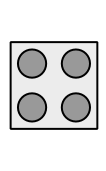
\includegraphics[height=6cm]{../../../lehre/folien_physik_projektpraktikum/legozeichnung.pdf}
% 	
\includegraphics[height=6cm]{../../../lehre/folien_praktikum_mechsys/pfeil.pdf}
% 	\includegraphics[height=6cm]{../../../lehre/folien_physik_projektpraktikum/fraese-lego-3d.png}
% 	
\includegraphics[height=6cm]{../../../lehre/folien_praktikum_mechsys/pfeil.pdf}
% 	\includegraphics[height=6cm]{../../../lehre/folien_physik_projektpraktikum/fraese-lego.png}
% 		
% 	\end{center}
% \end{frame}
% 
% \begin{frame}
% 	\frametitle{CNC-Drehbank}
% 	\begin{itemize}
% 		\item Material: z.B. Aluminium, POM
% 		\item Mehr oder weniger noch im Beta-Status
% 	\end{itemize}
% 		\begin{center}
% 	~\\
% 		\includegraphics[height=8cm]{../../../lehre/folien_physik_projektpraktikum/drehbank.png}
% 		~~~
% 		\includegraphics[height=8cm]{../../../lehre/folien_physik_projektpraktikum/drehstueck.png}
% 	\end{center}
% \end{frame}
% 
% \begin{frame}
% 	\frametitle{Elektrowerkstatt}
% 	\begin{itemize}
% 		\item Lötkolben, Oszi usw.
% 		\item Platinen selber fertigen:\\
% 			16x10\,cm, ein- oder doppelseitig -- technische Vorgaben beachten
% 		\item Minimaler Leiterbahnabstand: 8 mil
% 		\item Bauteileverkauf (ca. 350 gängige Typen)
% 	\end{itemize}
% 		\begin{center}
% 	~\\
% 		
\includegraphics[height=6cm]{../../../lehre/folien_praktikum_mechsys/schaltplan.pdf}
% 		
\includegraphics[height=6cm]{../../../lehre/folien_praktikum_mechsys/pfeil.pdf}
% 		\includegraphics[height=6cm]{../../werbung/bilder/Platine/platine_perspektivisch.png}
% 	\end{center}
% \end{frame}
% 
% %\hypersetup{colorlinks=true,urlcolor=blue}
% %\urlstyle{same}
% 
% \begin{frame}
% 	\frametitle{weitere Ausstattung}
% 	\begin{itemize}
% 		\item Werkzeug wie Schraubendreher, Feilen etc.
% 		\item Transferpresse
% 		\item Folienschneider
% 		\item Standbohrmaschine
% 		\item Nähmaschine
% 		\item Ofen
% 		\item Rechnerarbeitsplätze
% 		\item Grundausstattung an Software
% 		\item Grundstock an Material für alle Geräte
% 	\end{itemize}
% \end{frame}
% 
% \begin{frame}
% 	\frametitle{Interesse?}
% 	
% 	\begin{itemize}
% 		\item Ort: Hörsaalgebäude, beim unteren Ausgang H8/H9 (Erwin-Rommel-Straße 60, Raum U1.239)
% 		\item Öffnungszeiten: \\Ab zweiter Semesterwoche regelmäßig OpenLab
% 		% \item Workshops: Löten (Anfänger/Fortgeschrittene), 3D-Modellierung, usw.
% 		\item Weitere Termine auf {\color{blue} http://fablab.fau.de/termine}
% 		\item Auch Termine außerhalb der regulären Öffnungszeiten möglich!
% 	\end{itemize}
% 	~\\
% 	Motivation
% 	\begin{itemize}
% 		\item Mitgebrachte Werkstücke ansehen
% 		\item Flyer mitnehmen
% 	\end{itemize}
% 	~\\
% 	Fragen?
% 	\begin{itemize}
% 		\item Website {\color{blue} http://fablab.fau.de}
% 		\item E-Mail {\color{blue} kontakt@fablab.fau.de}
% 		\item Einfach vorbeikommen oder jetzt nachfragen
% 	\end{itemize}
% \end{frame}

% 
% \subsection{Second Subsection}

% \begin{frame}[plain]
% 	\begin{center}
% 		%\color{white}
% 		%\footnotesize
% 		~\\~\\~\\~\\~\\~\\~\\~\\~\\
% 		END
% 	\end{center}
% \end{frame}

\end{document}
